\subsubsubsubsection{Bus}
\begin{figure}[h]
\centering
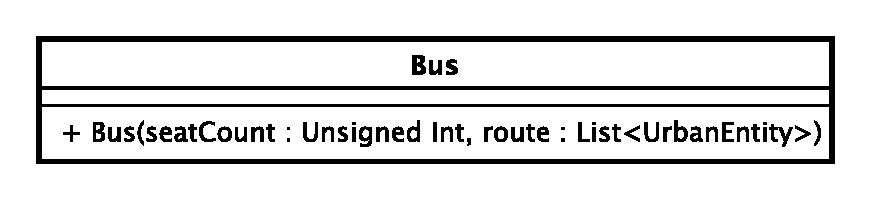
\includegraphics[scale=0.6,keepaspectratio]{images/solution/app/backend/bus.eps}
\caption{\pActive::Bus}
\label{fig:sd-app-bus}
\end{figure}
\FloatBarrier
\begin{itemize}
  \item \textbf{\descr} \\
It represents an entity that moves only on roadways and stops at each bus stop to
wait for passengers.
\item \textbf{\ops}
  \begin{itemize}
  \item[+] \texttt{Bus(seatCount : Unsigned Int, route : List<Infrastracture>)} \\
Creates a bus specifying its number of seats.
  \end{itemize}
\end{itemize} 
